\begin{frame}
\frametitle{Can we design a RemyCC that is TCP aware?}
\begin{table}
\begin{center}
\begin{tiny}
\begin{tabular}{l|l|l|l|l|l}
\bf RemyCC & \bf Link rates & \bf RTT & \bf Senders & ON/OFF time & Topology \\
\hline
TCP-aware  & 9--11~Mbps & 100~ms & \pbox{2.5cm}{2 Remy \\ 1 Remy, 1 AIMD}  & \pbox{2.5cm}{5 sec ON/OFF \\ 5 sec ON, 10 ms OFF} & Dumbbell\\
\hline
TCP-naive  & 9--11~Mbps & 100~ms & 2 Remy  & \pbox{2.5cm}{5 sec ON/OFF \\ 5 sec ON, 10 ms OFF} & Dumbbell\\
\hline
\end{tabular}
\end{tiny}
\caption{Training scenarios}
\label{table:oprange}
\end{center}
\end{table}

\begin{table}
\begin{center}
\begin{tiny}
\begin{tabular}{l|l|l|l|l}
\bf Link rates & \bf RTT & \bf Senders & ON/OFF time & Topology \\
\hline
10~Mbps & 100~ms & 2 TCP-aware & 5 sec ON, 10 ms OFF & Dumbbell\\
10~Mbps & 100~ms & 2 TCP-naive & 5 sec ON, 10 ms OFF & Dumbbell\\
10~Mbps & 100~ms & TCP-aware, AIMD & 5 sec ON, 10 ms OFF & Dumbbell\\
10~Mbps & 100~ms & TCP-naive, AIMD & 5 sec ON, 10 ms OFF & Dumbbell\\
10~Mbps & 100~ms & 2 AIMD  & 5 sec ON, 10 ms OFF & Dumbbell\\
\end{tabular}
\end{tiny}
\caption{Testing scenarios}
\label{table:oprange}
\end{center}
\end{table}

\end{frame}

\begin{frame}
\frametitle{RemyCC competing against itself}
\begin{centering}

\noindent \only<1>{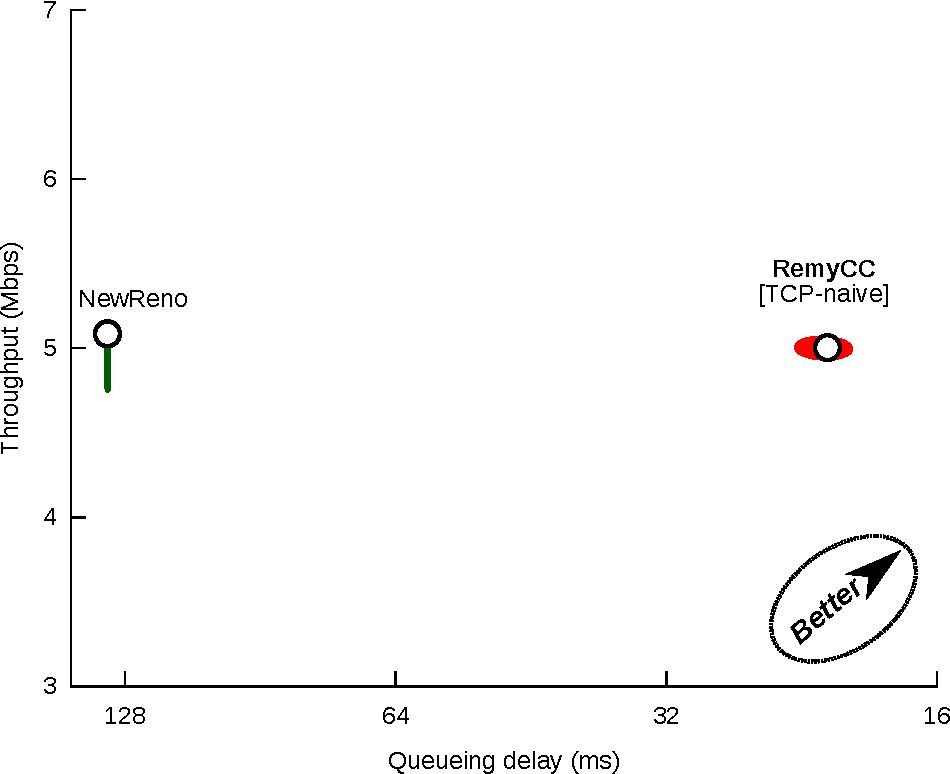
\includegraphics[width=3.3 in]{homo-1.pdf}}\only<2>{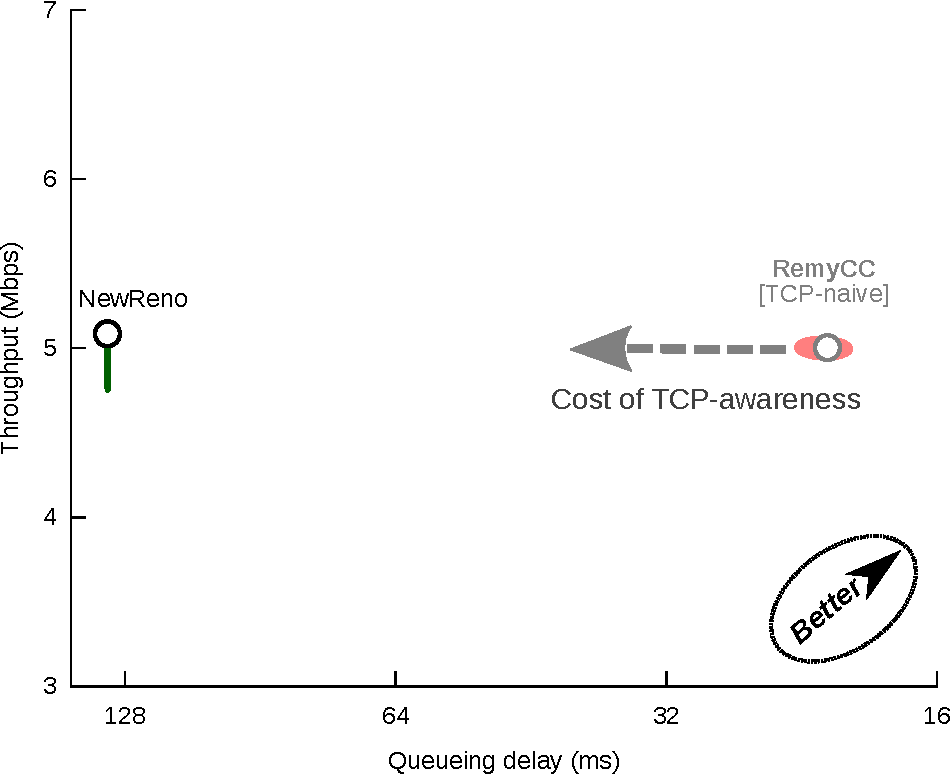
\includegraphics[width=3.3 in]{homo-2.pdf}}\only<3>{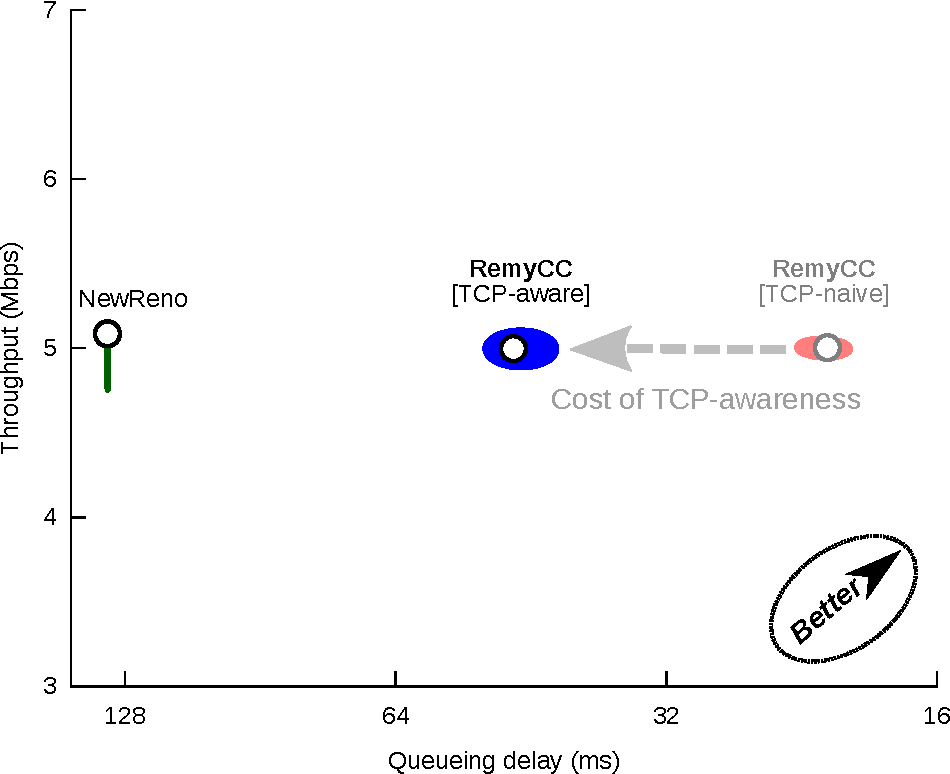
\includegraphics[width=3.3 in]{homo-3.pdf}}

\end{centering}
\end{frame}

\begin{frame}
\frametitle{RemyCC competing against TCP NewReno}
\begin{centering}

\noindent \only<1>{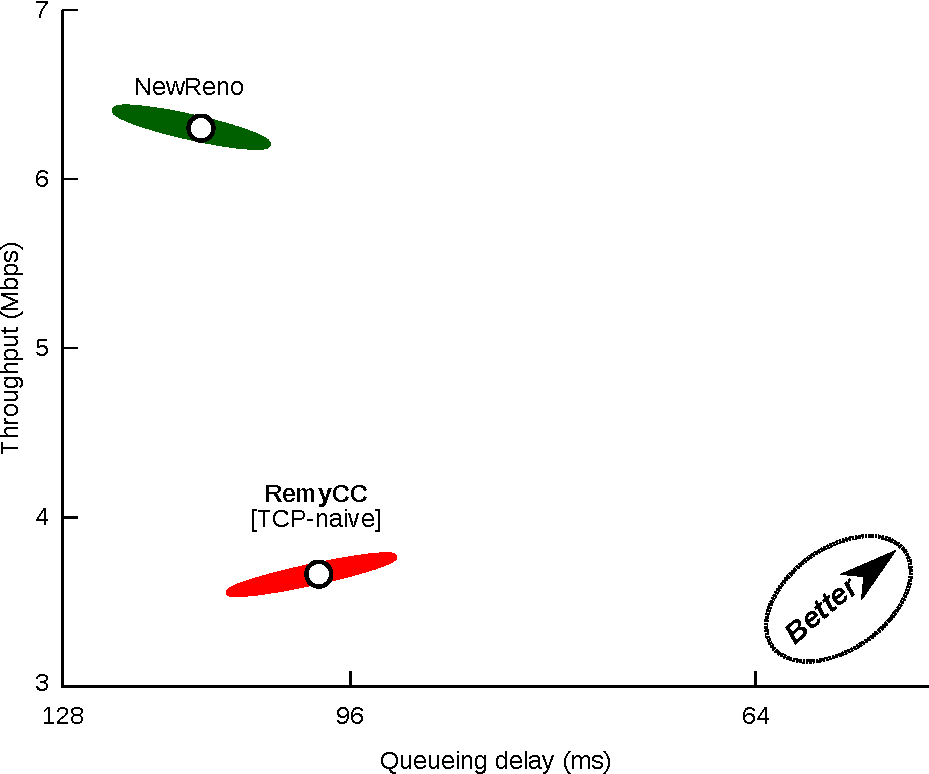
\includegraphics[width=3.3 in]{hetero-1.pdf}}\only<2>{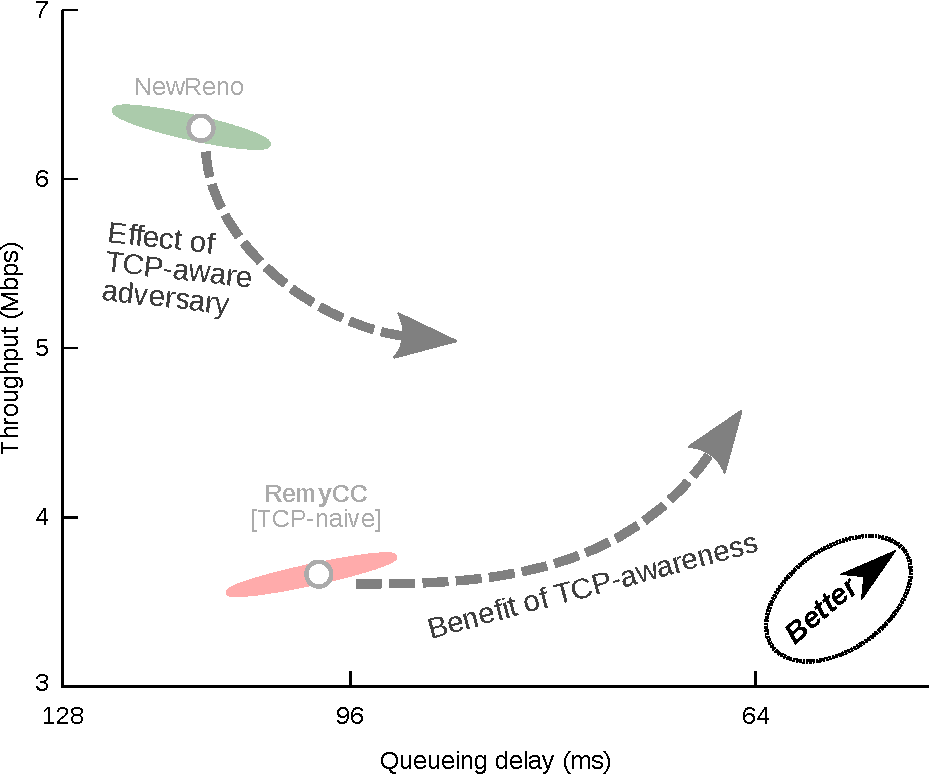
\includegraphics[width=3.3 in]{hetero-2.pdf}}\only<3>{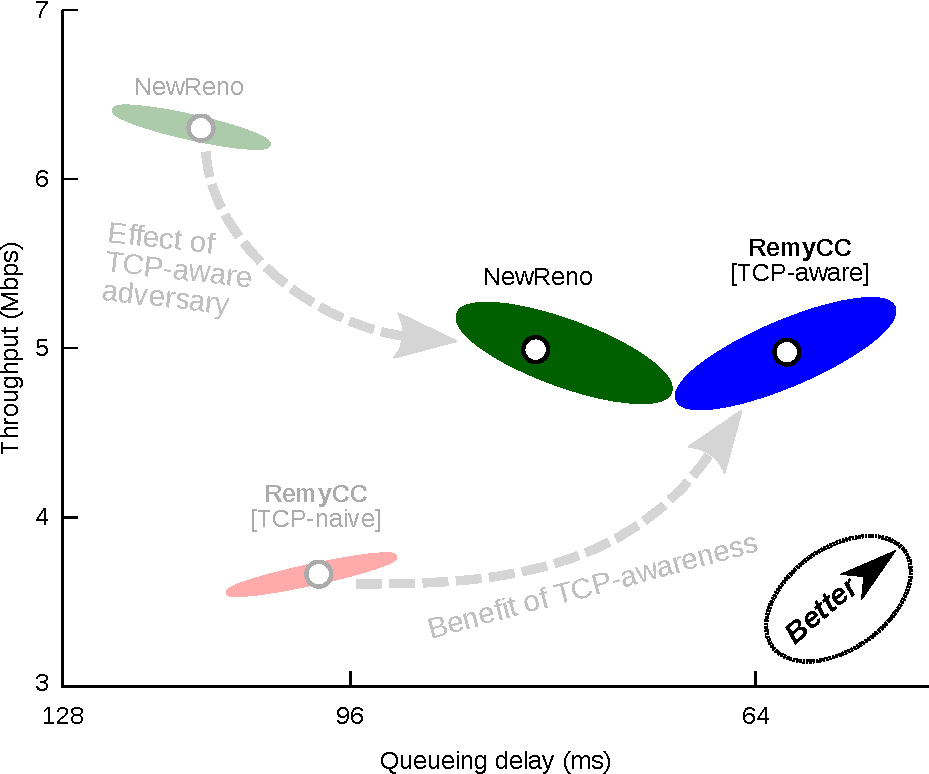
\includegraphics[width=3.3 in]{hetero-3.pdf}}

\end{centering}
\end{frame}
